\section{Zeichnen in \LaTeX}
\begin{frame}[fragile]{TikZ ist kein Zeichenprogramm}
\framesubtitle{Das Paket \pkg{tikz}}
Wir wollen nun mit \LaTeX{} ein wenig zeichnen. Dazu laden wir das Paket \pkg{tikz} und bei Bedarf durch \cmd{usetikzlibrary}\marg{Library 1,\dots,Library n} benötigte Bibliotheken für TikZ. 

\medskip\pause
Über die Umgebung \umg{tikzpicture} können wir nun anfangen mit TikZ ein Bild zu zeichnen. Von nun an stehen dem Benutzer eine ganze Reihe Befehle zur Verfügung. Der wichtigste ist hierbei \cmd{draw}\oarg{Options}. 
\end{frame}

\begin{frame}[fragile]{TikZ ist kein Zeichenprogramm}
\begin{block}{Verschiedene Formen}
\begin{tabular}{ll}
\verb+(0,0) -- (0,1)+ & Gerade von (0,0) bis (0,1)\\
\verb+(0,0) circle {r}+ & Kreis mit Radius r um (0,0)\\
\verb+(0,0) rectangle (1,1)+ & Rechteck zwischen (0,0) und (1,1)
\end{tabular}
\end{block}
\begin{block}{Optionen für \cmd{draw}}
\begin{tabular}{ll}
\verb+[->]+ & Kurven und Geraden werden zu Pfeilen\\
\verb+[thick]+ & Kurven und Geraden dick\\
\verb+[dashed]+ & Kurven und Geraden gestrichelt\\
\verb+[fill=red]+ & Inhalt wird rot eingefärbt\\
\end{tabular}\pause

Optionen können auch kombiniert werden. 
\end{block}
\end{frame}

\begin{frame}[fragile]{Beschriftung in TikZ}
\framesubtitle{Der Befehl \cmd{node}}
Wir wollen und können natürlich auch Beschriftungen ergänzen.

\medskip\pause
Der Befehl \cmd{node} ermöglicht dies. Syntax

\begin{center}
\cmd{node}\oarg{Positionierung} \texttt{at} \oarg{Coordinate} \marg{Text}
\end{center}

\medskip\pause
Hierbei genügt auch \cmd{node} \marg{Text} -- Beachte das Leerzeichen! 

\medskip\pause
Positionierung steht dann natürlich für \texttt{above}, \texttt{right}, \texttt{left}, etc. 
\end{frame}

\begin{frame}[fragile]{TikZ ist kein Zeichenprogramm}
\begin{columns}
\begin{column}{0.65\textwidth}
\begin{codeblock}
\begin{small}
\begin{verbatim}
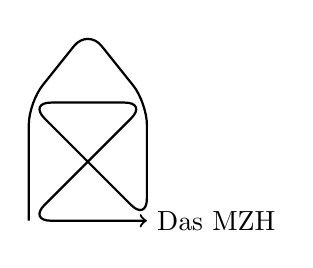
\begin{tikzpicture}[scale=.75]
\draw[thick, rounded corners=8pt,->] 
    (0,0) -- (0,2)
          -- (1,3.25)
          -- (2,2)
          -- (2,0)
          -- (0,2)
          -- (2,2)
          -- (0,0)
          -- (2,0) node[right] 
                  {Das MZH};
\end{tikzpicture}
\end{verbatim}
\end{small}
\end{codeblock}
\end{column}
\begin{column}{0.3\textwidth}
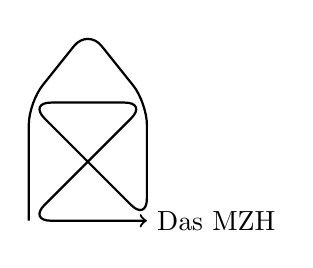
\begin{tikzpicture}[scale=.75]
\draw[thick, rounded corners=8pt,->] (0,0) -- (0,2)
                                           -- (1,3.25)
                                           -- (2,2)
                                           -- (2,0)
                                           -- (0,2)
                                           -- (2,2)
                                           -- (0,0)
                                           -- (2,0) node[right] {Das MZH};
\end{tikzpicture}
\end{column}
\end{columns}
\end{frame}
